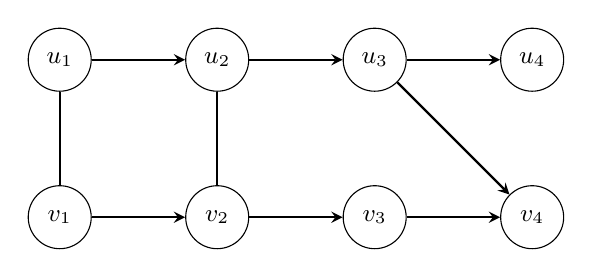
\begin{tikzpicture}[
    vertex/.style={circle, draw, minimum size=8mm, inner sep=0pt, font=\small},
    edge/.style={thick},
    dedge/.style={->, thick, >=stealth} % Directed edge style
]

    % Top horizontal path (first path)
    \node[vertex] (u1) at (0, 2) {$u_1$};
    \node[vertex] (u2) at (2, 2) {$u_2$};
    \node[vertex] (u3) at (4, 2) {$u_3$};
    \node[vertex] (u4) at (6, 2) {$u_4$};

    % Bottom horizontal path (second path)
    \node[vertex] (v1) at (0, 0) {$v_1$};
    \node[vertex] (v2) at (2, 0) {$v_2$};
    \node[vertex] (v3) at (4, 0) {$v_3$};
    \node[vertex] (v4) at (6, 0) {$v_4$};

    % Directed horizontal paths from left to right
    \draw[dedge] (u1) -- (u2);
    \draw[dedge] (u2) -- (u3);
    \draw[dedge] (u3) -- (u4);

    \draw[dedge] (v1) -- (v2);
    \draw[dedge] (v2) -- (v3);
    \draw[dedge] (v3) -- (v4);

    % Two vertical edges connecting the first two vertices of each path
    \draw[edge] (u1) -- (v1);
    \draw[edge] (u2) -- (v2);

    % One diagonal edge connecting the 3rd vertex of the 1st path and 4th vertex of the 2nd path
    \draw[dedge] (u3) -- (v4);

\end{tikzpicture}